\documentclass[10pt]{beamer}
\usepackage[utf8]{inputenc}
\usepackage[english]{babel}
\usepackage{alphabeta}
\usepackage{amsmath,amsthm,amsfonts,amssymb}
\usepackage[all,cmtip]{xy}
\usepackage{mathtools}
\usepackage{braket}
\usepackage[font=scriptsize,labelfont=bf]{caption}
\usepackage[english]{babel}
\usepackage{tikz}
\usepackage{xmpmulti}
\usepackage{soul}

% set colors
\definecolor{myNewColorA}{RGB}{0, 109, 174}
\definecolor{myNewColorB}{RGB}{111, 100, 169}
\definecolor{myNewColorC}{RGB}{0, 111, 41}

\setbeamercolor*{titlelike}{fg=myNewColorA}
\setbeamercolor*{title}{bg=myNewColorA, fg = white}
\setbeamercolor*{caption name}{fg=myNewColorA}

% references
\usepackage{natbib}
\usepackage{hyperref}

\newcommand*{\Scale}[2][4]{\scalebox{#1}{\ensuremath{#2}}}%
%------------------------------------------------------------

\setbeamerfont{title}{size=\large}
\setbeamerfont{subtitle}{size=\small}
\setbeamerfont{author}{size=\small}
\setbeamerfont{date}{size=\footnotesize}

\title{Faster than Hermitian time-evolution}
\subtitle{by Carl M Bender}
\author{Ana Fabela Hinojosa}
\institute[]{
\includegraphics[scale=0.18]{logo.jpg}}
\date[\today]{Supervisors:\\ Jesper Levinsen\\ Meera Parish } 
%------------------------------------------------------------
% This block of commands puts the table of contents at the 
% beginning of each section and highlights the current section:
\AtBeginSection[]
{
 \begin{frame}
    \frametitle{Contents}
    \tableofcontents[currentsection]
 \end{frame}
}

% ------Contents below------
%------------------------------------------------------------

\begin{document}

%The next statement creates the title page.
\frame{\titlepage}
\begin{frame}
\frametitle{Outline}
\tableofcontents
\end{frame}

%------------------------------------------------------------
\section{Introduction}
\begin{frame}{Hilbert space}
\vspace{1cm}

A Hilbert space is a vector space that can be infinite dimensional. \\
\vspace{1cm}
Vector spaces are equipped with an inner product. \\
\vspace{1cm}
Inner product:\\
    Defines a distance function. 

%  \vspace{-2cm}
\begin{figure}
    \hspace{6.5em}
    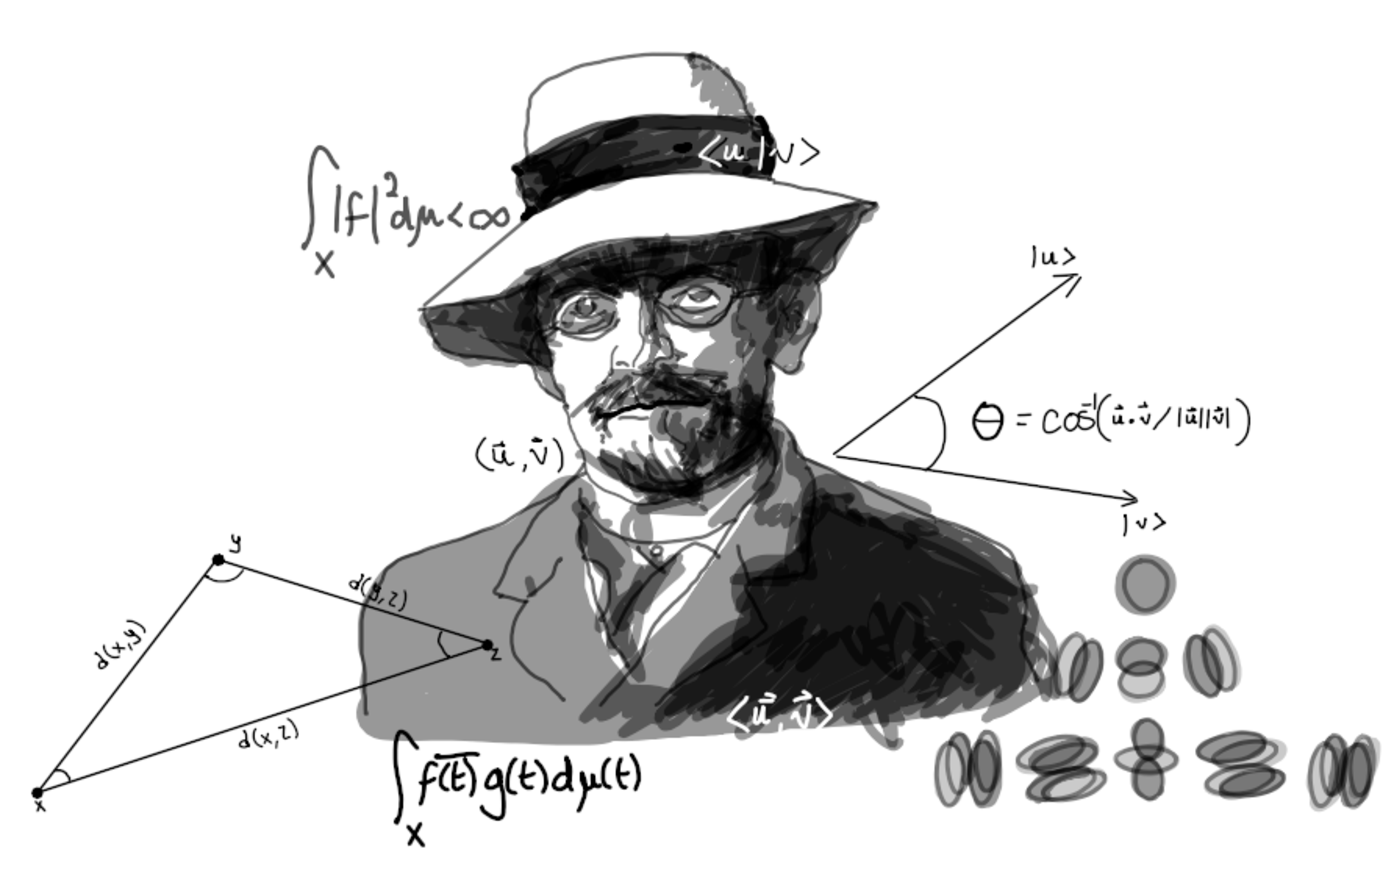
\includegraphics[width=0.7\textwidth]{hilbert.pdf}
    \\
    \tiny{Fig.3: Hilbert space stuff}
    \end{figure}
\end{frame}

% \begin{frame}{}
% \end{frame}

\begin{frame}{Hamiltonians as Observables}
    \centering{
    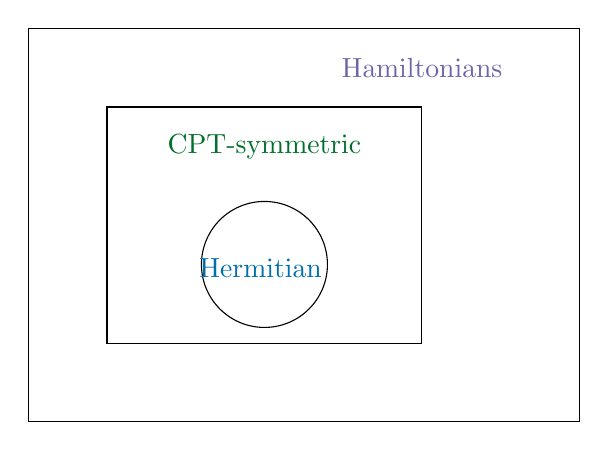
\begin{tikzpicture}
    \draw (-2,-1) rectangle(5,4) ++(-2,-0.5) node{\textcolor{myNewColorB}{Hamiltonians}};
    \draw (1,1) circle[x radius=0.8, y radius=0.8] ++(-0.05,-0.05) 
    node{\textcolor{myNewColorA}{Hermitian}};
    \pause
    \draw (-1,0) rectangle(3,3) ++(-2,-0.5) node{\textcolor{myNewColorC}{CPT-symmetric}};
    \end{tikzpicture}}
    \\
    \hspace{1em}
    \begin{tiny}
        Fig.1: The set of all possible Hamiltonians.
    \end{tiny}
    \\
    \begin{enumerate}
        \item \textcolor{myNewColorA}{Observables are \textbf{self-adjoint} operators $\{\hat{O}, \hat{H}, ...\}$}
        \item \textcolor{myNewColorC}{Real energy spectrum with defined lowest energy}
        \item \textcolor{myNewColorC}{A state $\psi$ of the quantum system is a unit vector of $\hat{H}$}
        \item \textcolor{myNewColorC}{Expectation values of observables are given by the inner-product.}
        \item \textcolor{myNewColorC}{Unitarity}
    \end{enumerate}
\end{frame}

\begin{frame}{Hamiltonians as Observables}
    \centering{
    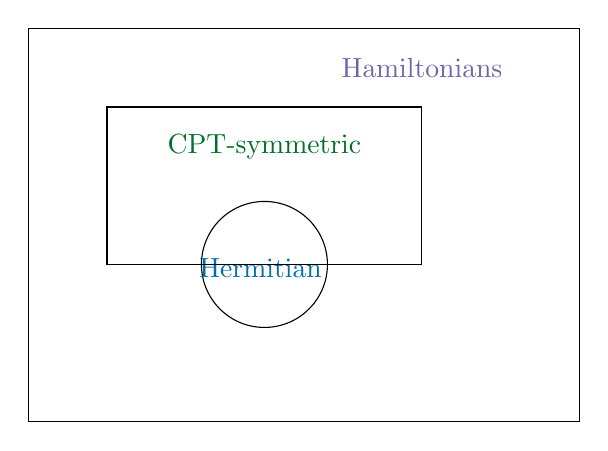
\begin{tikzpicture}
    \draw (-2,-1) rectangle(5,4) ++(-2,-0.5) node{\textcolor{myNewColorB}{Hamiltonians}};
    \draw (1,1) circle[x radius=0.8, y radius=0.8] ++(-0.05,-0.05) node{\textcolor{myNewColorA}{Hermitian}};
    \draw (-1,1) rectangle(3,3) ++(-2,-0.5) node{\textcolor{myNewColorC}{CPT-symmetric}};
    \end{tikzpicture}}
    \\
    \hspace{1em}
    \begin{tiny}
        Fig.1: The set of all possible Hamiltonians.
    \end{tiny}
    \\
    \begin{enumerate}
        \item \textcolor{myNewColorA}{\st{Observables are \textbf{self-adjoint} operators $\{\hat{O}, \hat{H}, ...\}$}}
        \item \textcolor{myNewColorC}{Real energy spectrum with defined lowest energy}
        \item \textcolor{myNewColorC}{A state $\psi$ of the quantum system is a unit vector of $\hat{H}$}
        \item \textcolor{myNewColorC}{Expectation values of observables are given by the inner-product.}
        \item \textcolor{myNewColorC}{Unitarity}
    \end{enumerate}
\end{frame}

\begin{frame}{CPT - symmetry}
\vspace{-2cm}
Hilbert space $\rightarrow \hat{H} = \hat{H}^{\mathcal{CPT}}$ \\
\begin{align*}
    & \mathcal{C} \rightarrow \mathrm{charge\:conjugation},\\
    & \mathcal{P} \rightarrow \mathrm{spatial\:inversion},\\
    & \mathcal{T} \rightarrow \mathrm{complex\:conjugation\:and\:time\:reversal}.
\end{align*}
\begin{align*}
    \hat{H}^{\mathcal{CPT}} = &\:\mathcal{CPT}\:\hat{H}\:\mathcal{CPT},\\
                            = & 
\end{align*}
inner product?
\end{frame}

\begin{frame}{Time evolution}
\vspace{-1cm}
\hspace{-2em}
\vspace{2cm}
\begin{columns}[T]
    \begin{column}{0.3\textwidth}
    \vspace{-2cm}
    \begin{align*}
    &\Scale[2]{\vec{\psi_{i}} \rightarrow{} \vec{\psi_{f}}}
    \end{align*}
    \pause
    \hspace{6em}
    \Scale[2.2]{\hookrightarrow}
    \end{column}
    
    \begin{column}{0.8\textwidth}
    \vspace{-1.3cm}
    \Scale[3]{\vec{\psi_{f}} = \hat{U} \vec{\psi_{i}}}\\
    \pause
    \hspace{6.8em}
    \begin{huge}
    {$\downarrow$}\\
    \end{huge}
    \begin{enumerate}
    \item \textcolor{myNewColorA}{Hermitian} quantum mechanics:\\
    \hspace{5em}
    $\hat{U} = e^{-i\hat{H}t / \hbar}$,\\
    \hspace{5em}
    where $t > 0$.
    \vspace{0.3cm}
    \pause
    \item \textcolor{myNewColorB}{non-Hermitian} quantum mechanics: \textcolor{myNewColorB}{\large{?}}
    \end{enumerate}
    \pause
    \vspace{0.7cm}
    \end{column}
    \end{columns}
\end{frame}

\section{Brachistochrone problem}
\begin{frame}{The Quantum Brachistochrone problem}
\vspace{0.5cm}
\begin{columns}
    \hspace{1.5em}
    \begin{column}{\textwidth}
    \multiinclude[format=png,start=1,graphics={width=0.5\textwidth}]
    {optim-gif/optimisation}
    \\
    \hspace{1em}
    \tiny{Fig.2:
    A particle travels from left to right in time t,\\
    \hspace{2.4em}
    Can we make this trip nearly instantaneous?}
    \end{column}
    
    \hspace{-15em}
    \begin{column}{0.5\textwidth}
    % \begin{equation*}
    % \mathrm{\beta\rho\alpha\chi\iota\sigma\tau\omicron\sigma\:\chi\rho\omicron\nu\omicron\sigma}
    % \end{equation*}
    \\
        brákhistos khrónos:\\
        ``shortest time"\\
    \vspace{1cm}
    \pause
    \small{\textcolor{myNewColorC}{How fast can we evolve?}
    }
    \end{column}
    \end{columns}
\end{frame}

\begin{frame}{The Quantum Brachistochrone problem}
\vspace{0.5cm}
\begin{columns}
    \hspace{1.5em}
    \begin{column}{\textwidth}
    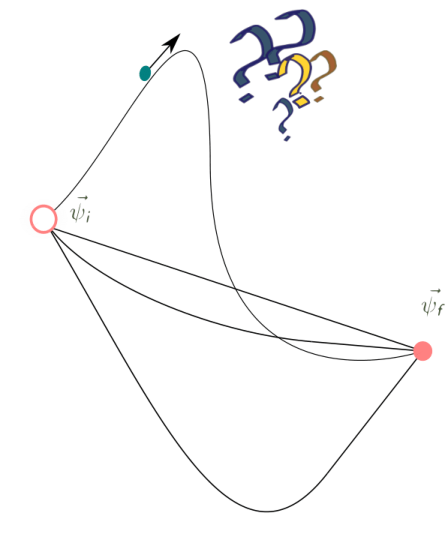
\includegraphics[width=0.5\textwidth]{optim-gif/optimisation-6}
    \\
    \hspace{1em}
    \tiny{Fig.2:
    A particle travels from left to right in time t,\\
    \hspace{2.4em}
    Can we make this trip nearly instantaneous?}
    \end{column}

    \hspace{-17em}
    \begin{column}{0.5\textwidth}
    \begin{enumerate}
        \item We want the shortest time step possible
        \pause
        % \item 
        % \pause
        \item \textcolor{myNewColorC}{Complex non-Hermitian Hamiltonians:\\ \quad time-optimal evolution}
        \pause
        % \item 
        % \pause
        \item \large{uncertainty principle violation?}
        \vspace{1cm}
    \end{enumerate}
    \end{column}
    \end{columns}
\end{frame}

\begin{frame}{The Maths}
\begin{columns}
    \hspace{1.5em}
    \begin{column}{\textwidth}
    \textcolor{myNewColorA}{Hermitian} case
    \hspace{-1.5em}
    \begin{equation*}
    \hat{H}  = \begin{pmatrix}
                s & r e^{-i\theta}  \\
                r e^{i \theta} & u  \\
                \end{pmatrix} , \quad \{r, s, \theta, u\} \in \mathbb{R}
    \end{equation*}\\
    Time evolution
    \hspace{-1.5em}
    \begin{equation*}
    \vec{\psi_f}  = \hat{U} \vec{\psi_i}
    \end{equation*} \\
    energy constraint
    \hspace{-1.5em}
    \begin{equation*}
     \omega^2 = (s-u)^2 + 4r^2
    \end{equation*} \\
    \end{column}
\end{columns}
\end{frame}

\begin{frame}{The Maths}
\begin{columns}
    \hspace{1.5em}
    \begin{column}{\textwidth}
    \textcolor{myNewColorC}{CPT-symmetric} case
    \hspace{-1.5em}
    \begin{equation*}
    \Tilde{H}  = \begin{pmatrix}
                r e^{i\theta} & s  \\
                s & r e^{-i\theta}  \\
                \end{pmatrix}, \quad \{r, s, \theta\} \in \mathbb{R}
    \end{equation*}\\
    Time evolution
    \hspace{-1.5em}
    \begin{equation*}
    \vec{\psi_f}  = \hat{U} \vec{\psi_i}
    \end{equation*} \\
    energy constraint
    \hspace{-1.5em}
    \begin{equation*}
     \omega^2 = 4s^2 - 4r^2 \sin^2{\theta}
    \end{equation*} \\
    \end{column}
\end{columns}
\end{frame}

% \begin{frame}{}
% \end{frame}

% \begin{frame}{}
% \end{frame}

\section{Conclusion}
\begin{frame}{Conclusion}
\end{frame}

\begin{frame}{References} 
    \nocite{*}
    \bibliographystyle{unsrturl_mod}
    \bibliography{mybib.bib}
\end{frame}

\section{Appendix}
\begin{frame}{Appendix}
\end{frame}

\end{document}





